$y=x^3$, $y=0$, $x=2;x=2$.

\nopagebreak
\begin{align*}
\text{Región acotada por } y=x^3, y=0, x=2. \text{ Rotación alrededor de } x=2. \\
\text{Usamos el método de capas cilíndricas (shells).} \\
\text{Radio } r = 2-x, \text{ Altura } h = x^3. \\
V &= \int_{0}^{2} 2\pi (2-x) x^3 \, dx \\
&= 2\pi \int_{0}^{2} (2x^3 - x^4) \, dx \\
&= 2\pi \left[ \frac{x^4}{2} - \frac{x^5}{5} \right]_{0}^{2} \\
&= 2\pi \left( \frac{16}{2} - \frac{32}{5} \right) = 2\pi \left( 8 - 6.4 \right) \\
&= 2\pi (1.6) = 3.2\pi = \frac{16\pi}{5}
\end{align*}

\[
\boxed{\displaystyle \frac{16\pi}{5}}
\]

\begin{center}
    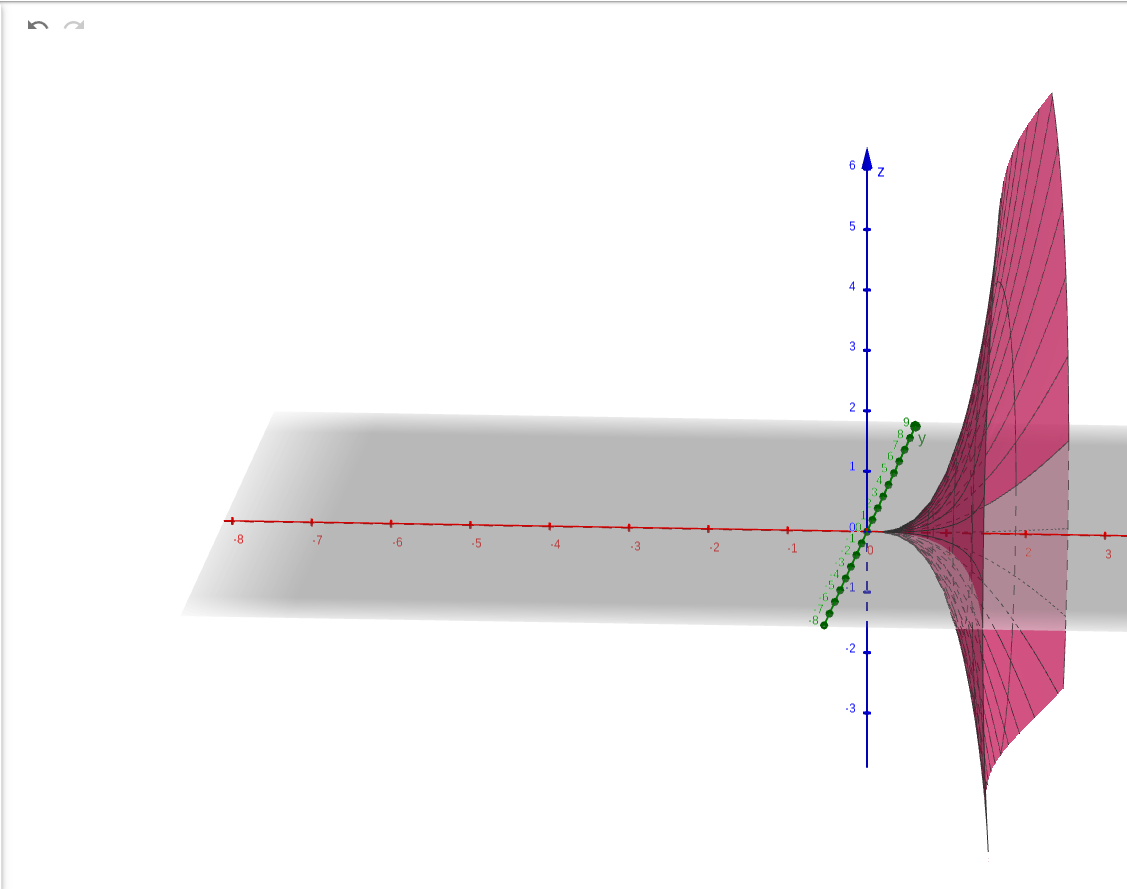
\includegraphics[width=0.5\textwidth]{Graficas/ejer29.png}
\end{center}
